\section{Introduction}
\label{sec:intro}

Task-specific  conversational  chatbot  \cite{wen2016network}  has been applied
into  many practical products. One typical example is the chatbot that shares the working burden of
human  customer  service  agents  responsible  for  customers' questions. 
Another one is the speech-based control in
devices  like  intelligent  speakers, such as Siri, Google home, Baidu Xiaodu,
and smart home equipments, to name a few. Regardless of whether these conversations belong to
single or  multi-round, an essential technique underlying this type of chatbot is to
identify  the  real  intention  behind  a  user's  question or reply. 
The detected intention  with  its  associated  information  is then mapped into a
predefined dialog logic graph, from which a suitable response (e.g., conducting 
expected actions, replying texts or accomplishing some operations, etc)  is returned.
This  is  the  main  difference  from  a  free chatbot.  

Intention detection in task-specific chatbot  is  a  challenging task due to its inherent properties. First,
a customer's  utterance  within  a conversation is usually quite short. Since it
does  not  contain  enough  information,  short  texts \cite{song2014short} are
thought  to  be  more  ambiguous  compared to long texts such as paragraphs or
documents,  posing  a  great challenge \cite{chen2019deep} for classification
task   \cite{phan2008learning,yan2009dynamic,hua2015short}.   Second,  in  the
initial  stage  of  building  a  chatbot , it is often rather hard to collect
sufficient  labeled  data  to  train  a good model. Developers have to
examine tons of real system logs for typical user's utterances, and then label
them  with expected intentions. Therefore, to build a task-specific chatbot with
high  performance, it is essential to solve the challenge of short-text
classification   \cite{sriram2010short}   problem   under   few-shot   setting
\cite{yu2018diverse}.


Generally  there  are  two  kinds  of  approaches  to  address  this  problem,
one is based on the \emph{text classification model} that directly maps an input text into a most likely label, and
the other one is based on the \emph{text similarity  model}  that searches the most similar text to the input and returns the associated label.


\emph{Text classification}  includes  classic  long  text
classification  and  short  text  classification  in  this  scenario.  Besides
traditional  machine  learning  models  like  SVM \cite{suykens1999least},  
boosting  tree \cite{tu2005probabilistic},  many work
\cite{wen2016network}  choose  neural  network  such  as  convolutional neural
networks (CNNs) \cite{kim2014convolutional,zhang2015character,conneau2016very}
and       long       short       term       memory       networks      (LSTMs)
\cite{mousa2017contextual,liu2016recurrent}   to   accomplish   the   task  of
extracting  semantic  features from limited amount of words. Their common model
structure  is  adding  a  softmax classifier as the final layer to predict the
labels.  Another  two  interesting lines of work, label-word joint models, and
joint  NER  and  classification  are  discussed  in  the related work section.
Recently,   pre-trained   language   models   on   large  corpus  like  BERT
\cite{devlin2018bert}  and  RoBERTa \cite{liu2019roberta} has been proven more
powerful  in  solving  many  NLP  tasks  including  short-text  classification
\cite{madabushi2020cost}.      Especially      for      few-shot     scenarios
\cite{yu2018diverse},     pre-trained     models    based    on    transformers
\cite{vaswani2017attention} tends to be more helpful to alleviate the dearth of training data.

\emph{Text similarity model}  is usually employed to calculate the similarities between an input text 
and historical texts in the repository, and returns the associated label of the historical
text with highest similarity score. 
One of the state-of-the-art similarity models is based on multiple cross-attention
mechanism  \cite{barkan2020scalable}.
Due to the   fact   that   many   experiment   results   have   shown   that  RoBERTa
\cite{liu2019roberta} is an improved version of BERT \cite{devlin2018bert}, and has achieved amazing
results  on  both  text  classification and text similarity-related
tasks, we choose RoBERTa as one of the baselines in this paper.

%\emph{Text similarity model}  is also called sentence-pair model. 
%Its  motivation  originates  from  the idea of retrieval based
%chatbot   \cite{jafarpour2010filter,   leuski2011npceditor}.   Given  a dataset consists of
%Question-Answer (QA)  pairs and a user query Q, the retrieval based conversational
%system will search from the dataset  the most matched pair (Q', A') 
%through  semantic  analysis  and  return  A'  as  the  answer  to Q
%\cite{mnasri2019recent}. In this way, sentence-pair model pre-trained on large
%corpus  can be employed  to  identify  the class with highest semantic similarity to
%customer's    query.    A    common    model    structure    of    pre-trained 
%sentence-pair model is based on multiple cross-attention
%mechanism  \cite{barkan2020scalable}. Due to
%the   fact   that   many   experiment   results   have   shown   that  RoBERTa
%\cite{liu2019roberta} is an improved version of BERT \cite{devlin2018bert}, and has achieved amazing
%results  on  both  text  classification and sentence-pairs semantic similarity
%tasks, we choose RoBERTa as one of the baselines in this paper.

Despite  the  success  of  these two kinds of approaches, they still have some
limitations   in   task-specific  chatbot  scenario.  As  for  the  \emph{text
classification  model},  it  is  not  easy to use data augmentation method to
solve  the  data insufficiency challenge. It is usually unfeasible to
get  large amount of domain-specific data when facing a new task. With respect
to  the  \emph{similarity model}, though we can obtain a large amount of data
through similar sentence detection  \cite{sun2019fine},  it  is  still  quite  hard  to  perform well on
a new task-specific dataset,  since their objective losses are totally different. 

The  above  limitations motivate us to propose a joint system that is capable of
taking  advantages  from both the classification and similarity models. We call
it  as SFC,  short  for  similarity model fused with classification model, shown in
Fig.  \ref{fig:framework}.  We further bring in multi-task learning   \cite{caruana1993multitask,collobert2008unified,  liu2019multi} to train SFC.  
Our basic  idea  consists of two stages. In the first stage, we use an auxiliary model
to  select  top-K most possible labels for an input. This model can be an elastic
search  \cite{divya2013elasticsearch}  or a text classification model trained on
current   task-specific   chatbot   data.  In  the  second  stage,  we  build  a
classification  model  whose  main  modules  are  similarity  models. Then, this
structure  derives  two  goals to train towards, the classification loss for our
application,  and  the similarity loss for the main modules. When the two stages
are  independently optimized, we call \emph{two-stage SFC}. We further find that
the  quality of the output from the first stage might limit the final performance of the
system,  since  the  candidate labels for each user query is always fixed in the
whole  multi-task  training  process.  This  observation motivates us to further
improve  the  two-stage  SFC  into a joint training setting, called \emph{joint SFC}. In
this  way,  the  candidate texts associated  with the top-K classes also become
dynamic,  and  the  text  classification  model  in the first stage will also be
further optimized to provide better top-K results by the final training loss.


We summarize our contributions as follows:
\begin{enumerate}
  \item We propose a novel joint system to makes full use of
  the advantages from both the text classification and similarity models.

  \item To  better  train such a system, we bring in multi-task training to obtain
  reasonable performance.

  \item Experiment  results  from 4 public and 1 private short-text classification
  datasets,  show  that  our  proposed  SFC joint system can achieve significant
  and consistent improvements over strong baselines, especially in the low resource settings.
\end{enumerate}

\begin{figure*}[t]
  \begin{centering}
    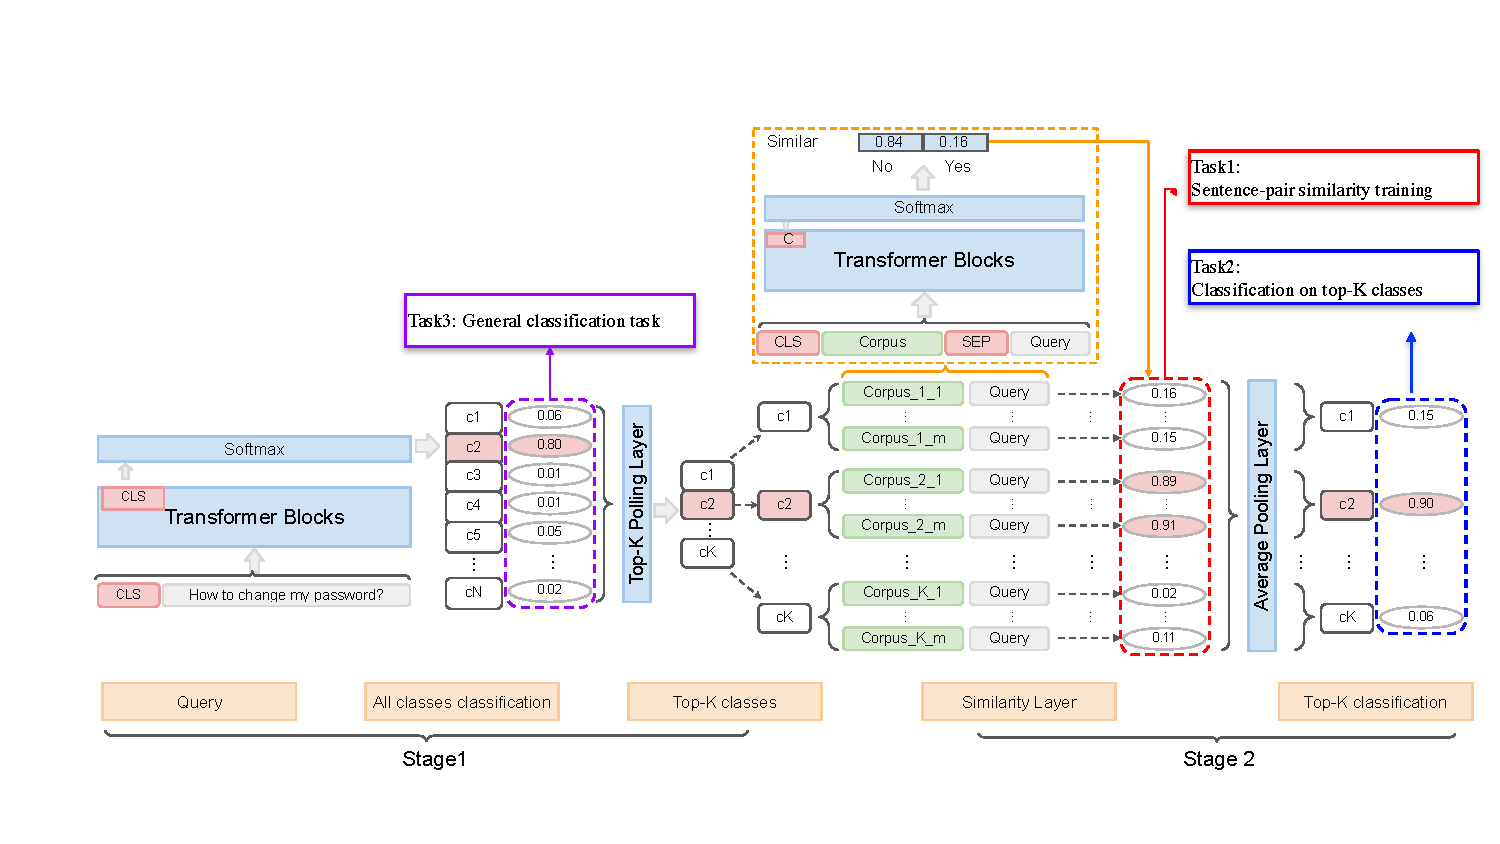
\includegraphics[scale=0.72]{picture/picture4} 
    \par
  \end{centering}
  \caption{
    \textbf{Network Structure of SFC:} two-stage SFC and joint-SFC are sharing
    the  same  network  from  stage  1  and  stage 2, with the only difference
    whether two stages being jointly trained.
  }
  \label{fig:framework}
\end{figure*}

